\documentclass[12pt, a4paper] {ncc}
\usepackage[utf8] {inputenc}
\usepackage[T2A]{fontenc}
\usepackage[english, russian] {babel}
\usepackage[usenames,dvipsnames]{xcolor}
\usepackage{listings,a4wide,longtable,amsmath,amsfonts,graphicx,tikz}
\usepackage{indentfirst,fancyvrb,pdfpages,tabularx}
\usepackage[rounded]{syntax}

\begin{document}
\setcounter{figure}{0}
\frenchspacing
\pagestyle{empty}
% ============================ ТИТУЛЬНЫЙ ЛИСТ ================================
\begin{center}
     Национальный исследовательский университет информационных технологий,
                              механики и оптики.\\
                       Кафедра систем управления и информатики.\\
                  Основы теории автоматического управления.
\end{center}
\vspace{\stretch{2}}
\begin{center}
                         {\bf Лабораторная работа №5}\\
                Свободное и вынужденное движение линейных систем.\\
                                {\sl 5 вариант}
\end{center}
\vspace{\stretch{3}}
\begin{flushright}
                                    Студент:\\
                                    {\it Куклина М.Д., P3401}\\
                                    Преподаватель: \\
                                    {\it Кремлев А.С.}
\end{flushright}
\vspace{\stretch{4}}
\begin{center}
                                      2018
\end{center}
% ======================== КОНЕЦ ТИТУЛЬНОГО ЛИСТА ============================
\newpage
\pagestyle{plain}
% ================================ ОТЧЁТ =====================================

\section{Задание}

Начальные условия и корни характеристических уравнений:

\begin{center}
\begin{tabularx}{0.8\textwidth}{|c|X|X|X|X|}
\hline
$N$ & \multicolumn{2}{c|}{Начальные условия} & \multicolumn{2}{c|}{Корни характеристического} \\
    & \multicolumn{2}{c|}{}                  & \multicolumn{2}{c|}{уравнения} \\
\cline{2-5}
    & $y_0$  & $\dot{y_0}$ & $\lambda_1$  & $\lambda_2$  \\
\hline
1   & $1$    & $0$         & $-2.0$       & $-2.0$       \\
2   & $1$    & $0$         & $-0.9 + j7$  & $-0.9 + j7 $ \\
3   & $1$    & $0$         & $j7 $        & $-j7 $       \\
4   & $0.05$ & $0$         & $0.9 + j7 $  & $0.9 - j7 $  \\
5   & $0.05$ & $0$         & $2.0$        & $2.0$        \\
6   & $0$    & $0.1$       & $-0.5$       & $0.5$        \\
\hline
\end{tabularx}
\end{center}

Параметры системы и входное воздействие:

\begin{center}
\begin{tabular}{|c|c|c|c|c|c|}
\hline
$a_0$ & $a_1$ & $b$ & $g_1(t)$ & $g_2(t)$ & $g_3(t)$ \\
\hline
3 & 3 & 2 & $2.0$ & $0.8t$ & $\sin(3t)$ \\
\hline
\end{tabular}
\end{center}

\section{Математическая модель и схема моделирования}

\begin{figure}[ht!]
\begin{center}
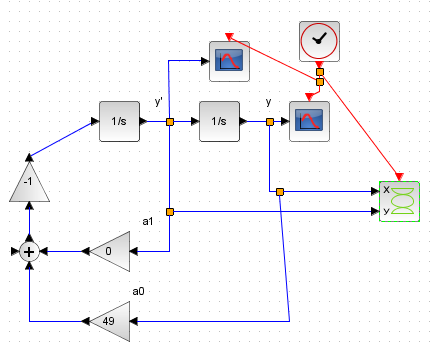
\includegraphics[width=0.4\textwidth]{scheme}
\end{center}
\caption*{Схема моделирования свободной составляющей}
\end{figure}
\subsection{Поиск $a_0$, $a_1$}

Нам даны два корня уравнения $\lambda^2 + a_1 \lambda + a_0 = 0$. Подставляя их
в уравнение, имеем систему:

\begin{equation*}
    \left\{
        \begin{aligned}
            \lambda_1^2 + a_1 \lambda_1 + a_0 &= 0 \\
            \lambda_2^2 + a_1 \lambda_2 + a_0 &= 0
        \end{aligned}
    \right.
\end{equation*}

Имеем по теореме Виета:

\begin{equation*}
    \begin{aligned}
        a_0 &= \lambda_1 \lambda_2 \\
        a_1 &= - \left(\lambda_1 + \lambda_2\right)
    \end{aligned}
\end{equation*}

\subsection{Поиск выражения свободной составляющей}

В зависимости от корней характеристического уравнения свободная составляющая
может принимать разный вид:

\subsubsection{Корни веществены и одинаковы: $\lambda_1 = \lambda_2 = \lambda$}

    \begin{equation*}
        y_\text{св} (t) = \left(C_1 + C_2 t\right) e^{\lambda t}
        \Rightarrow
            \left\{\begin{aligned}
            y_\text{св}  (0) &= C_1 \\
            y'_\text{св} (0) &= \lambda C_1 + C_2 \\
            \end{aligned}\right.
        \Rightarrow
            \left\{\begin{aligned}
            C_1 &= y_\text{св}(0) \\
            C_2 &= - \lambda y_\text{св}(0) + y'_\text{св}(0)
            \end{aligned}\right.
    \end{equation*}

    \begin{equation*}
    y_\text{св} (t) = \left(y_\text{св}(0) \cdot (1 - \lambda t) + y'_\text{св}(0) t\right) e^{\lambda t}
    \end{equation*}

\subsubsection{Корни веществены и различны: $\lambda = \alpha \pm (\beta + 0i)$}

    \begin{equation*}
        y_\text{св} (t) = C_1 e^{\lambda_1 t} + C_2 e^{\lambda_2 t}
        \Rightarrow
        \left\{\begin{aligned}
        y_\text{св}  (0) &= C_1 + C_2 \\
        y'_\text{св} (0) &= \lambda_1 C_1 + \lambda_2 C_2 \\
        \end{aligned}\right.
        \Rightarrow
        \left\{\begin{aligned}
        C_1 &= \dfrac{y'_\text{св}(0) - \lambda_2 y_\text{св}(0)}{\lambda_1 - \lambda_2} \\
        C_2 &= -\dfrac{y'_\text{св}(0) - \lambda_1 y_\text{св}(0)}{\lambda_1 - \lambda_2} \\
        \end{aligned}\right.
    \end{equation*}

    \begin{equation*}
        y_\text{св} (t) = \dfrac{1}{\lambda_1 - \lambda_2} \left( \left(y'_\text{св}(0) - \lambda_2 y_\text{св}(0)\right) e^{\lambda_1 t} -
        \left(y'_\text{св}(0) - \lambda_1 y_\text{св}(0)\right) e^{\lambda_2 t}\right)
    \end{equation*}

\subsubsection{Корни комплексные: $\lambda = \alpha \pm \omega i$}

\begin{equation*}
y_\text{св} (t) = A e^{\alpha t} \sin(\omega t + \phi)
\Rightarrow
\left\{\begin{aligned}
y_\text{св}  (0) &= A \sin(\phi) \\
y'_\text{св} (0) &= A \left( \omega \cos(\phi) + \alpha \sin(\phi)\right) \\
\end{aligned}\right.
\Rightarrow
\end{equation*}
\begin{equation*}
\left\{\begin{aligned}
\phi &= \arcctg \left( \omega^{-1} \cdot \left( \dfrac{y'_\text{св}(0)}{y_\text{св}(0)} - \alpha \right) \right) \\
A &= y_\text{св} (0) \cdot \text{sgn}\left(y'_\text{св}(0) - \alpha y_\text{св}(0)\right)
	\sqrt{\left( \omega^{-1} \cdot \left( \dfrac{y'_\text{св}(0)}{y_\text{св}(0)} - \alpha \right) \right)^2 + 1}
\end{aligned}\right.
\end{equation*}

\subsubsection{Корни комплексные и число мнимые: $\lambda = \pm \omega i$}

Применяя наработки предыдущего параграфа при $\alpha = 0$:

    \begin{equation*}
        y_\text{св} (t) = A \sin(\omega t + \phi)
        \Rightarrow
        \left\{\begin{aligned}
        y_\text{св}  (0) &= A \sin(\phi) \\
        y'_\text{св} (0) &= A \omega \cos(\phi) \\
        \end{aligned}\right.
        \Rightarrow
        \left\{\begin{aligned}
        \phi &= \arcctg \left( \dfrac{y'_\text{св}(0)}{\omega y_\text{св}(0)} \right) \\
        A &= y_\text{св} (0) \cdot \text{sgn}\left(y'_\text{св}(0)\right)
        	\sqrt{\left(\dfrac{y'_\text{св}(0)}{\omega y_\text{св}(0)}\right)^2 + 1}
        \end{aligned}\right.
    \end{equation*}


\section{Расчёт}

\begin{center}
\begin{tabularx}{0.95\textwidth}{|c|X|X|X|X|X|X|c|}
\hline
$N$ & \multicolumn{2}{c|}{Корни}  & \multicolumn{2}{c|}{Параметры} & \multicolumn{2}{c|}{Условия} & Свободная \\
\cline{2-7}
    & $\lambda_1$    & $\lambda_2$        & $a_0$    & $a_1$  & $y_0$  & $\dot{y_0}$ & составляющая $y_\text{св}(t)$\\
\hline
1   & $-2  $         & $-2  $             & $4$     & $4$    & $1$    & $0$       & $(1+2t)e^{-2t} $                        \\ \hline
2   & \multicolumn{2}{c|}{$-0.9 \pm j7 $} & $49.81$ & $-1.8$    & $1$    & $0$    & $ 1.0082 e^{-0.9t} \sin(7t + 1.443)$           \\ \hline
3   & \multicolumn{2}{c|}{$\pm j7 $}      & $49$    & $0$    & $1$    & $0$       & $ \sin(7t + \frac {\pi}{2})$             \\ \hline
4   & \multicolumn{2}{c|}{$0.9 \pm j7 $}  & $49.81$ & $1.8 $    & $0.05$ & $0$    & $ 0.05041 e^{0.9t} \sin(7t - 1.443)$ \\ \hline
5   & $2  $          & $2  $              & $4$     & $-4$    & $0.05$ & $0$      & $ (1 - 2t) e^{2t}$                      \\ \hline
6   & \multicolumn{2}{c|}{$\pm 0.5$}      & $-0.25 $& $0$  & $0$    & $0.1$       & $ -0.1e^{-0.5t} + 0.1e^{0.5t} $  \\ \hline
\end{tabularx}
\end{center}
% a0 = l1 l2 a1 = - (l1 + l2)
\section{Эксперименты}

\subsection{Расчёт свободных составляющих}

\subsubsection{Эксперимент 1}

$y$:
\begin{center}
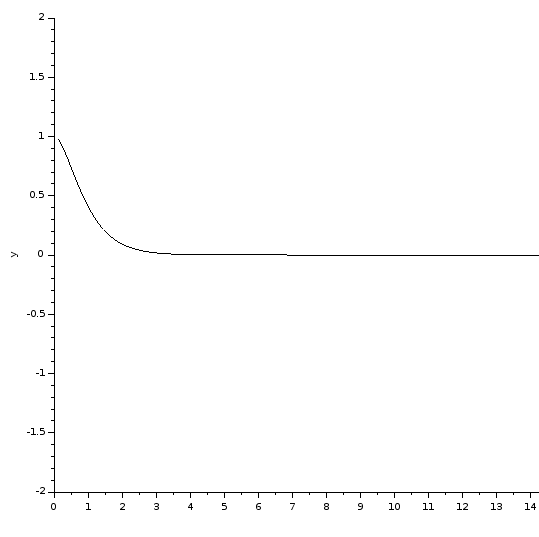
\includegraphics[width=0.5\textwidth]{1y}
\end{center}

$y'$:
\begin{center}
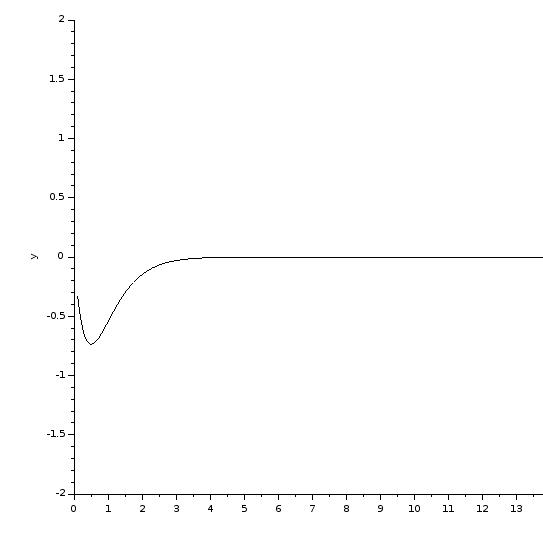
\includegraphics[width=0.5\textwidth]{1y1}
\end{center}

\subsubsection{Эксперимент 2}

$y$:
\begin{center}
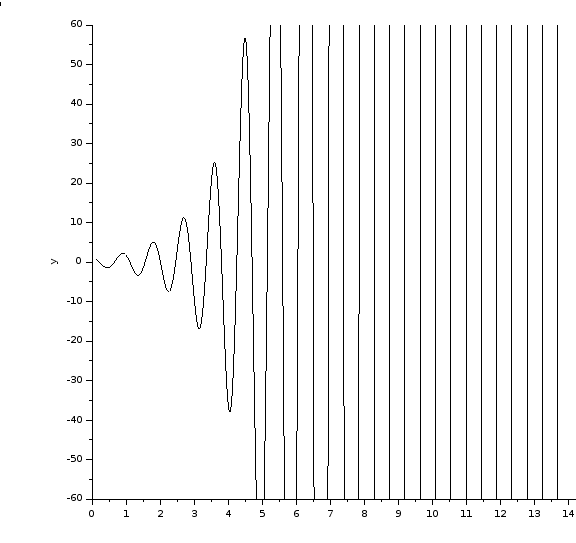
\includegraphics[width=0.5\textwidth]{2y}
\end{center}

$y'$:
\begin{center}
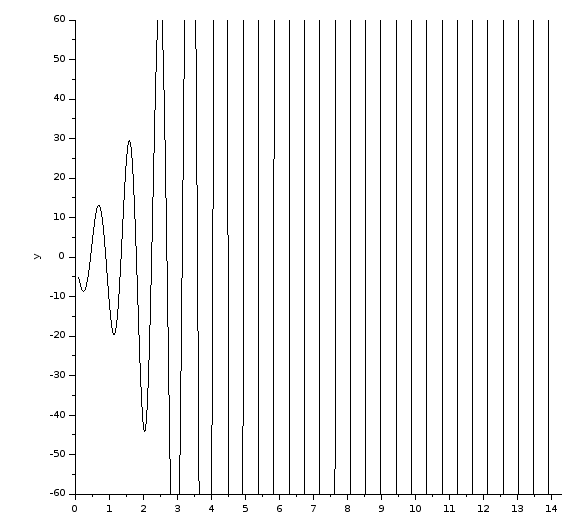
\includegraphics[width=0.5\textwidth]{2y1}
\end{center}

\subsubsection{Эксперимент 3}

$y$:
\begin{center}
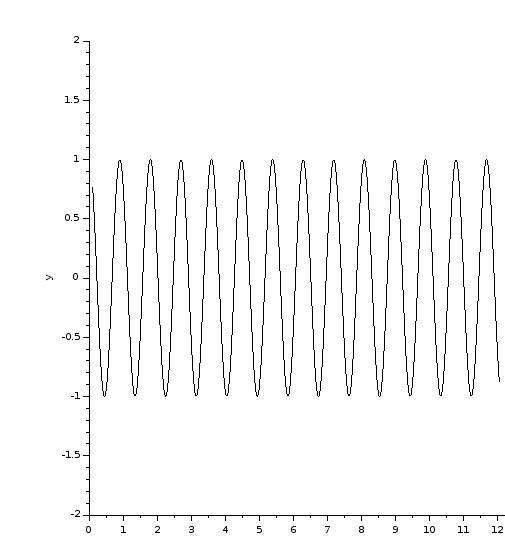
\includegraphics[width=0.5\textwidth]{3y}
\end{center}

$y'$:
\begin{center}
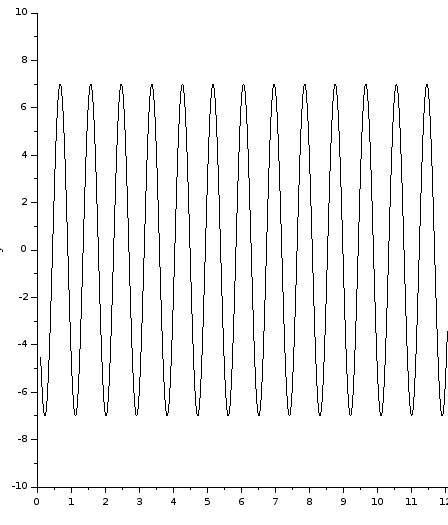
\includegraphics[width=0.5\textwidth]{3y1}
\end{center}

\subsubsection{Эксперимент 4}

$y$:
\begin{center}
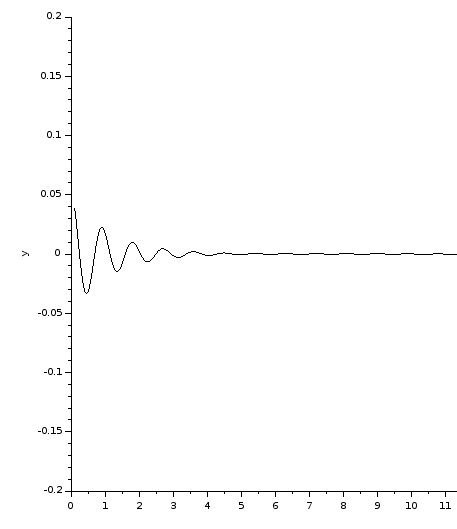
\includegraphics[width=0.5\textwidth]{4y}
\end{center}

$y'$:
\begin{center}
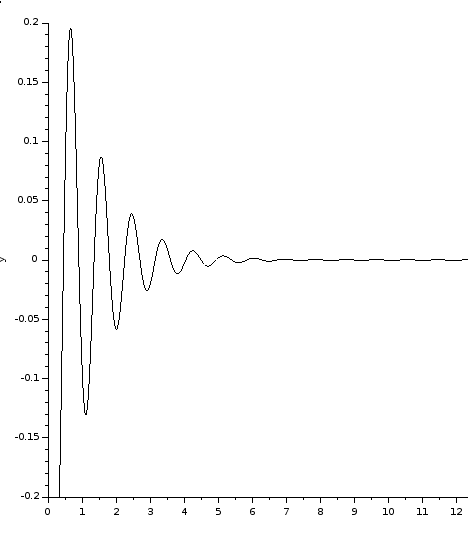
\includegraphics[width=0.5\textwidth]{4y1}
\end{center}

\subsubsection{Эксперимент 5}

$y$:
\begin{center}
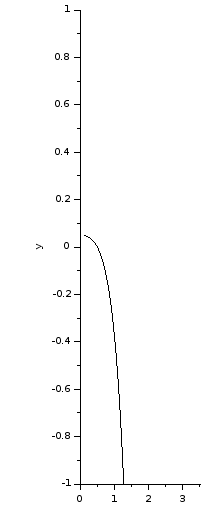
\includegraphics[width=0.2\textwidth]{5y}
\end{center}

$y'$:
\begin{center}
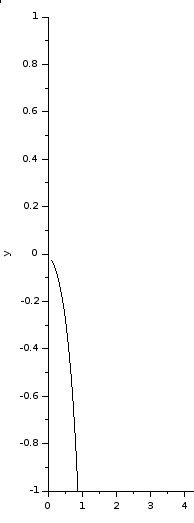
\includegraphics[width=0.2\textwidth]{5y1}
\end{center}

\subsubsection{Эксперимент 6}

$y$:
\begin{center}
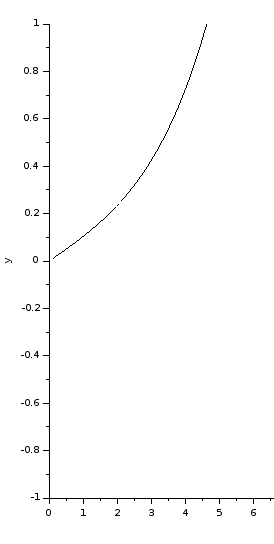
\includegraphics[width=0.3\textwidth]{6y}
\end{center}

$y'$:
\begin{center}
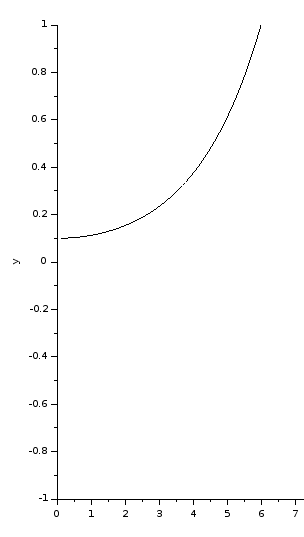
\includegraphics[width=0.3\textwidth]{6y1}
\end{center}

\subsection{Фазовые кривые}
\subsubsection{ $ 1.0082 e^{-0.9t} \sin(7t + 1.443)$}

\begin{center}
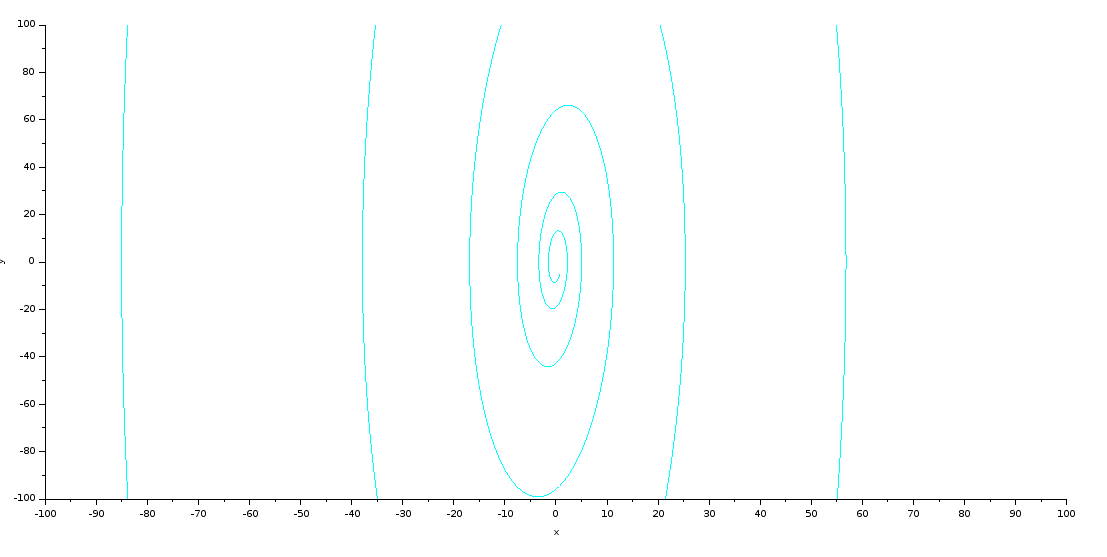
\includegraphics[width=0.6\textwidth]{1f}
\end{center}

\subsubsection{  $ \sin(7t + \frac {\pi}{2})$}
\begin{center}
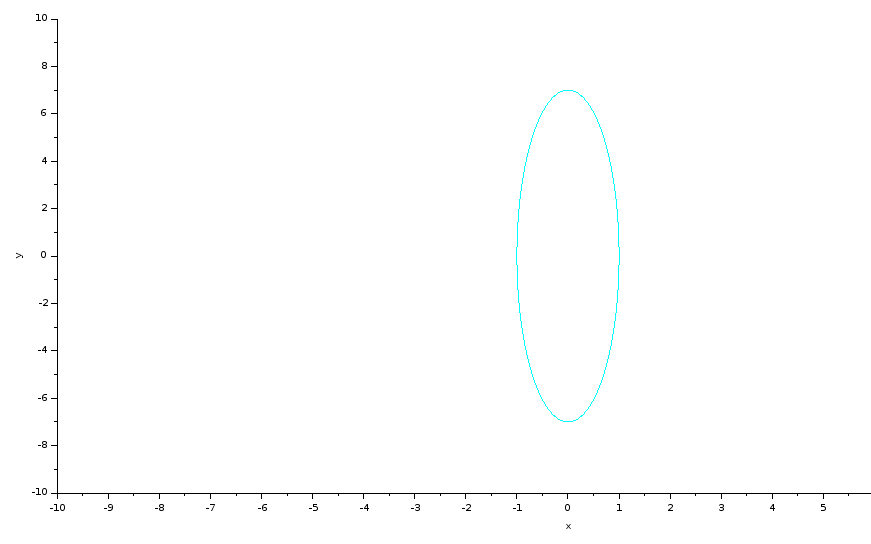
\includegraphics[width=0.6\textwidth]{2f}
\end{center}

\subsubsection{ $ 0.05041 e^{0.9t} \sin(7t - 1.443)$}
\begin{center}
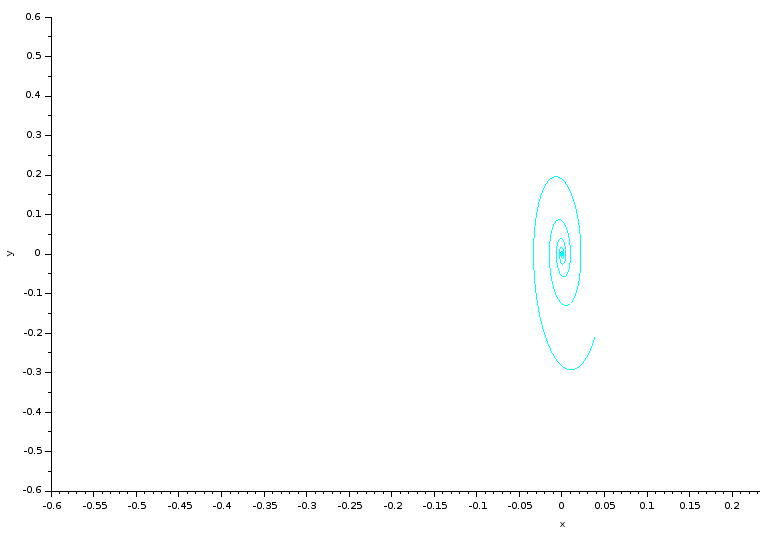
\includegraphics[width=0.6\textwidth]{3f}
\end{center}

\subsection{Вынужденное движение}

\subsubsection{$g_1 = 2.0$}

\paragraph{Для условия $y(0) = -1$}
\begin{center}
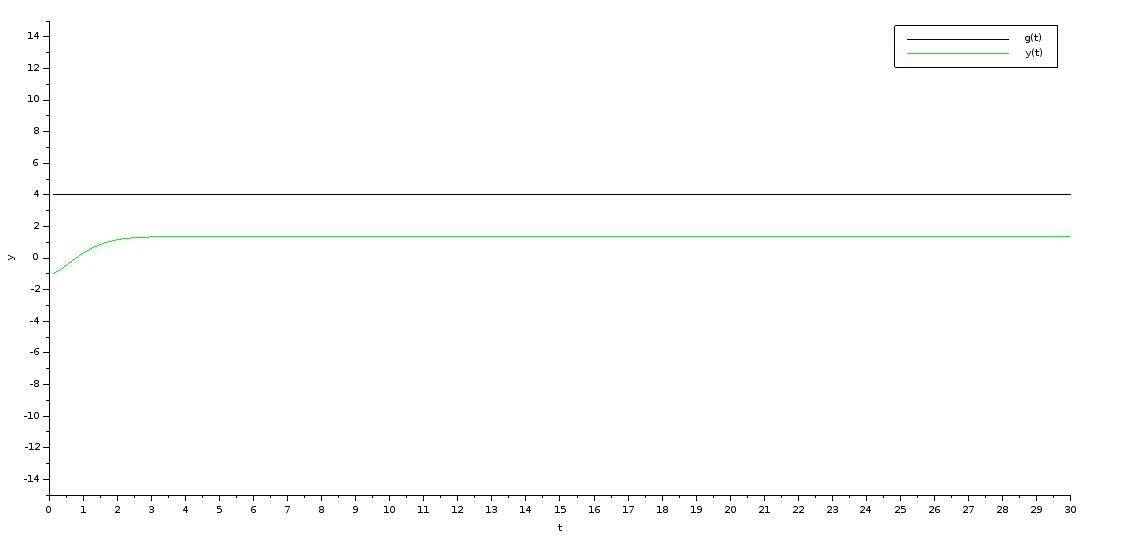
\includegraphics[width=0.9\textwidth]{g-1.png}
\end{center}

\paragraph{Для условия $y(0) = 0$}
\begin{center}
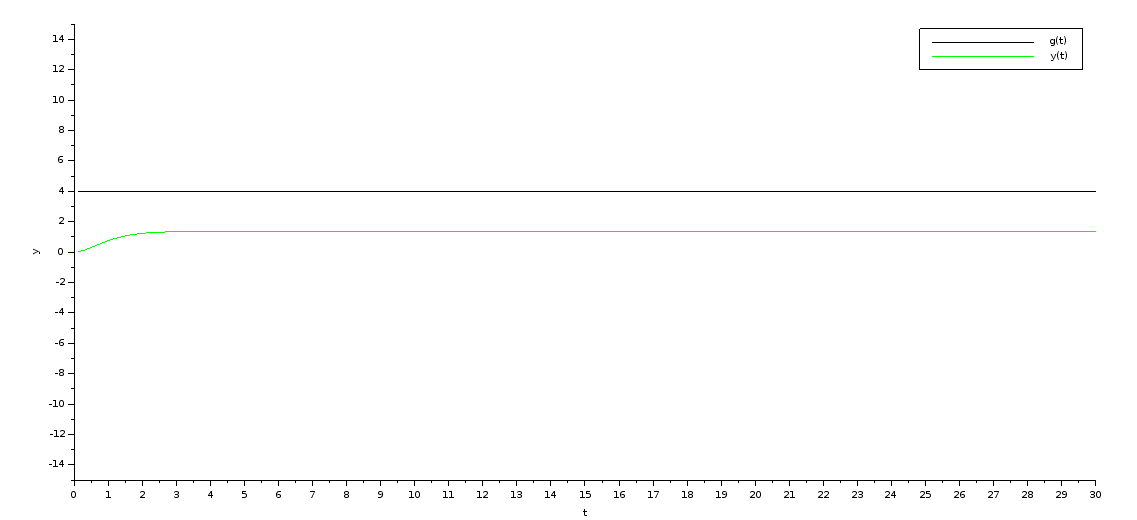
\includegraphics[width=0.9\textwidth]{g0.png}
\end{center}

\paragraph{Для условия $y(0) = 1$}
\begin{center}
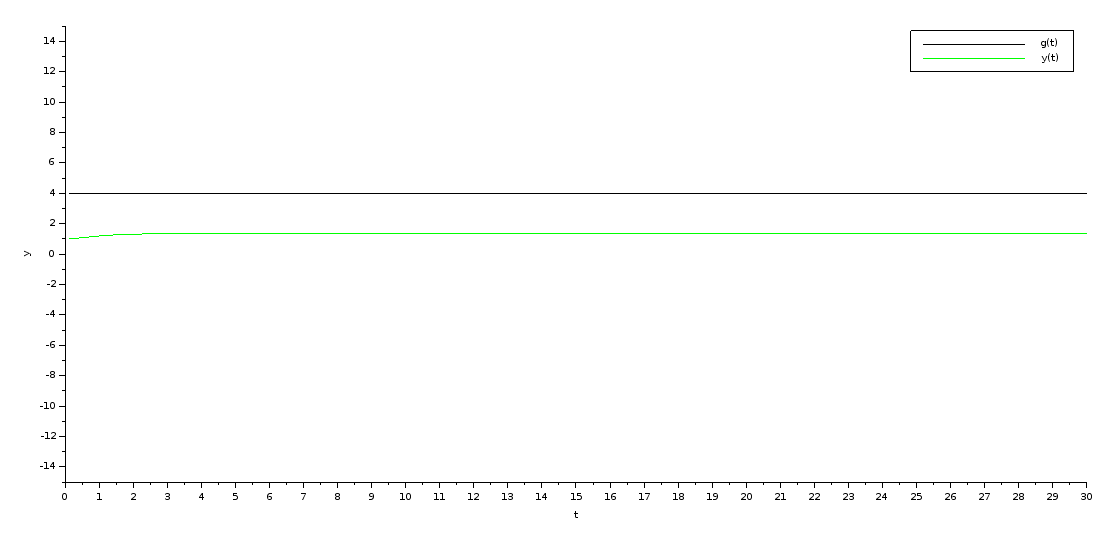
\includegraphics[width=0.9\textwidth]{g1.png}
\end{center}

\subsubsection{$g = 0.8t$}
\paragraph{Для условия $y(0) = -1$}
\begin{center}
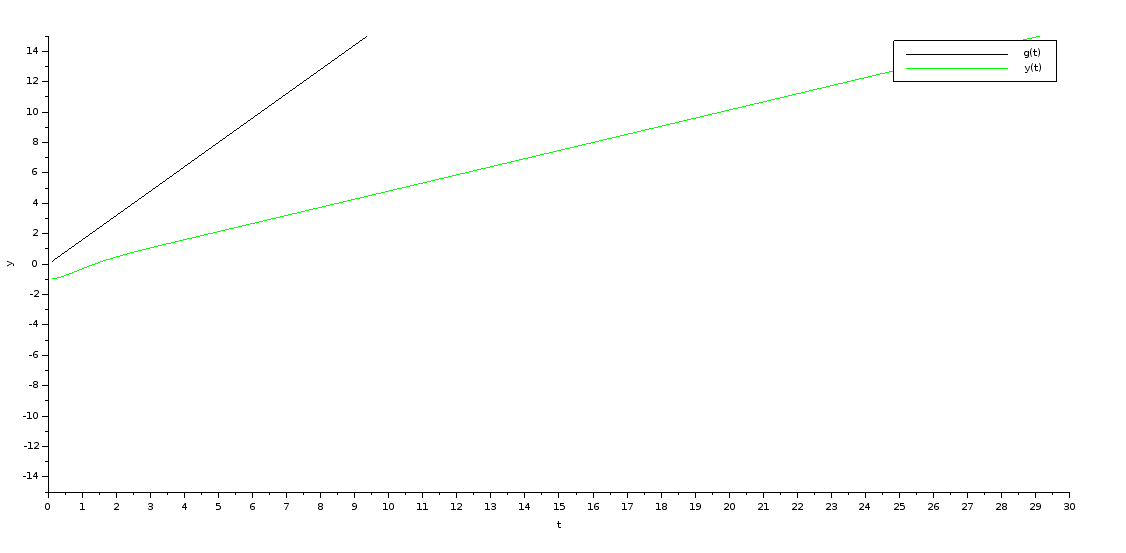
\includegraphics[width=0.9\textwidth]{2g-1.png}
\end{center}

\paragraph{Для условия $y(0) = 0$}
\begin{center}
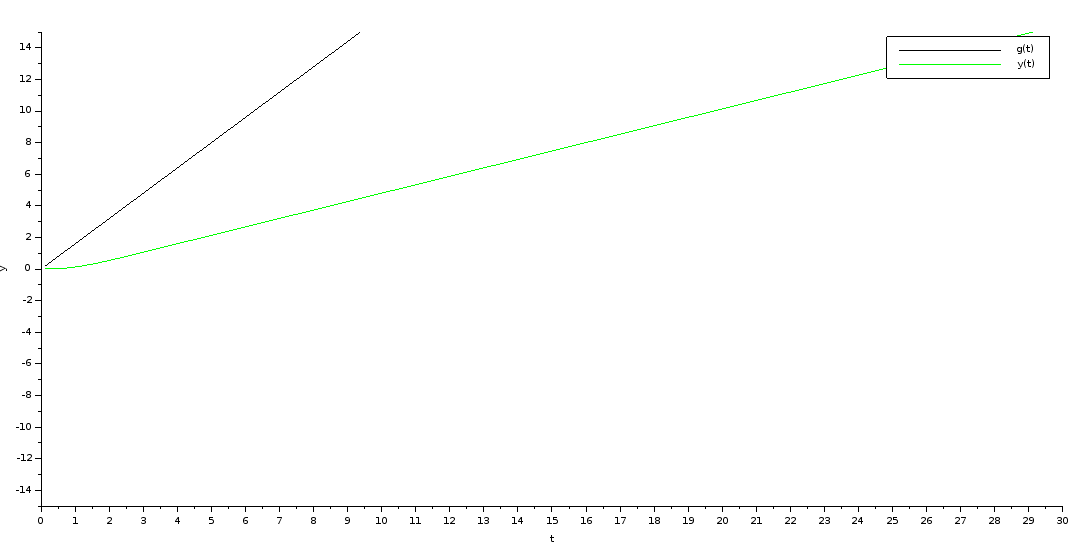
\includegraphics[width=0.9\textwidth]{2g0.png}
\end{center}

\paragraph{Для условия $y(0) = 1$}
\begin{center}
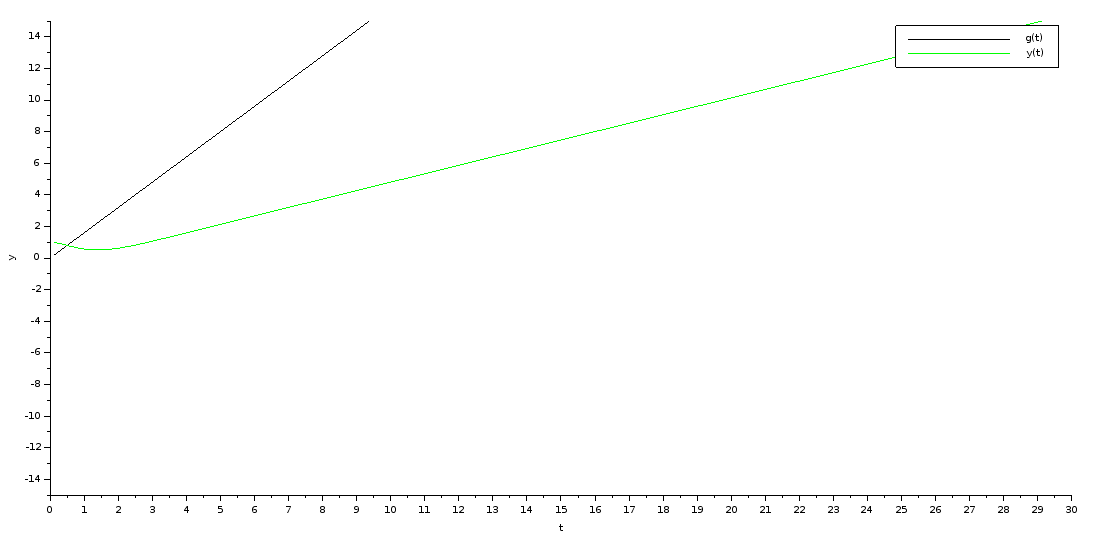
\includegraphics[width=0.9\textwidth]{2g1.png}
\end{center}

\subsubsection{$g = \sin(3t)$}

\paragraph{Для условия $y(0) = -1$}
\begin{center}
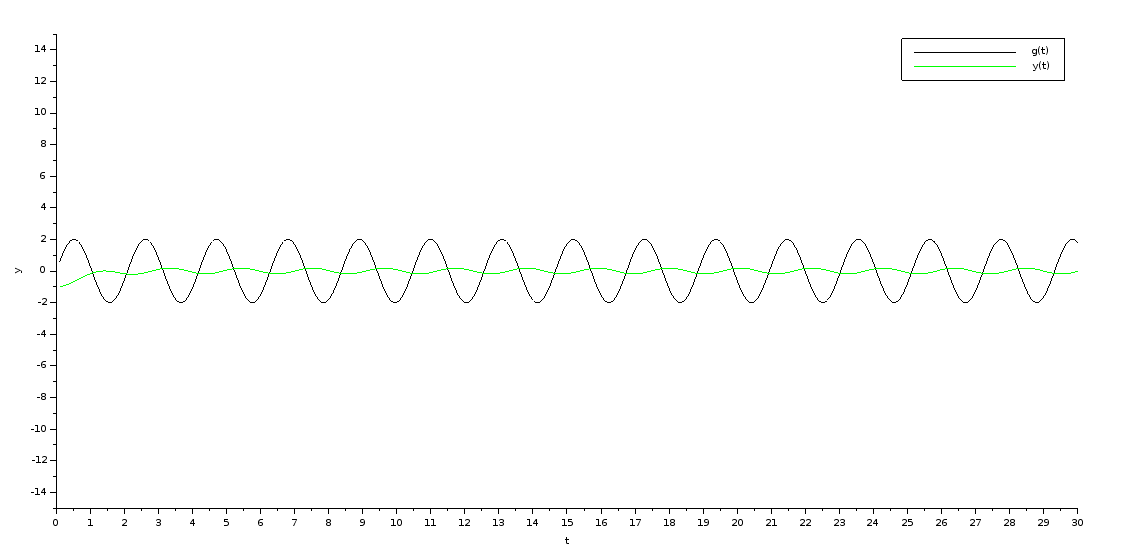
\includegraphics[width=0.9\textwidth]{3g-1.png}
\end{center}

\paragraph{Для условия $y(0) = 0$}
\begin{center}
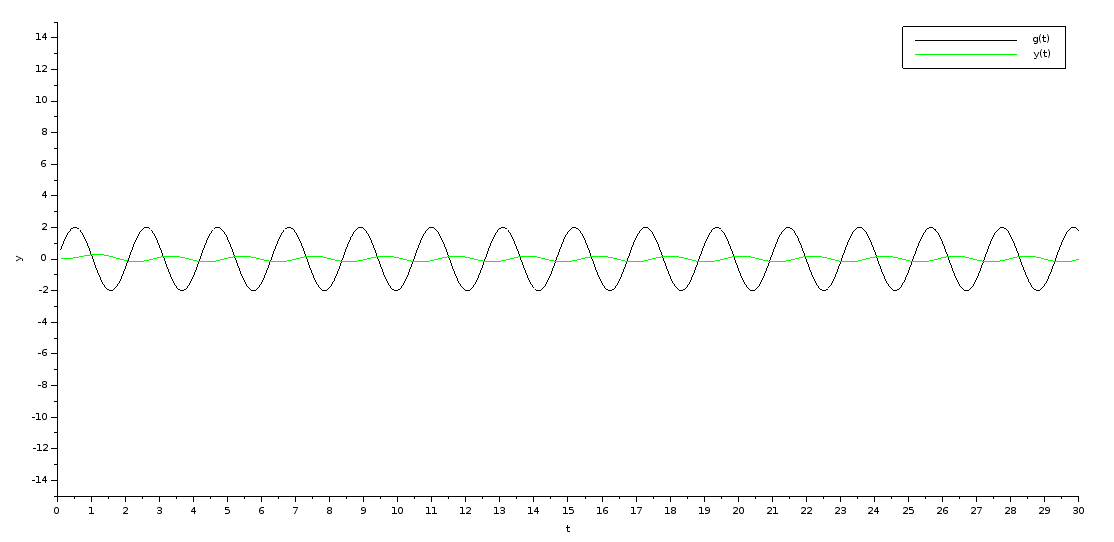
\includegraphics[width=0.9\textwidth]{3g0.png}
\end{center}

\paragraph{Для условия $y(0) = 1$}
\begin{center}
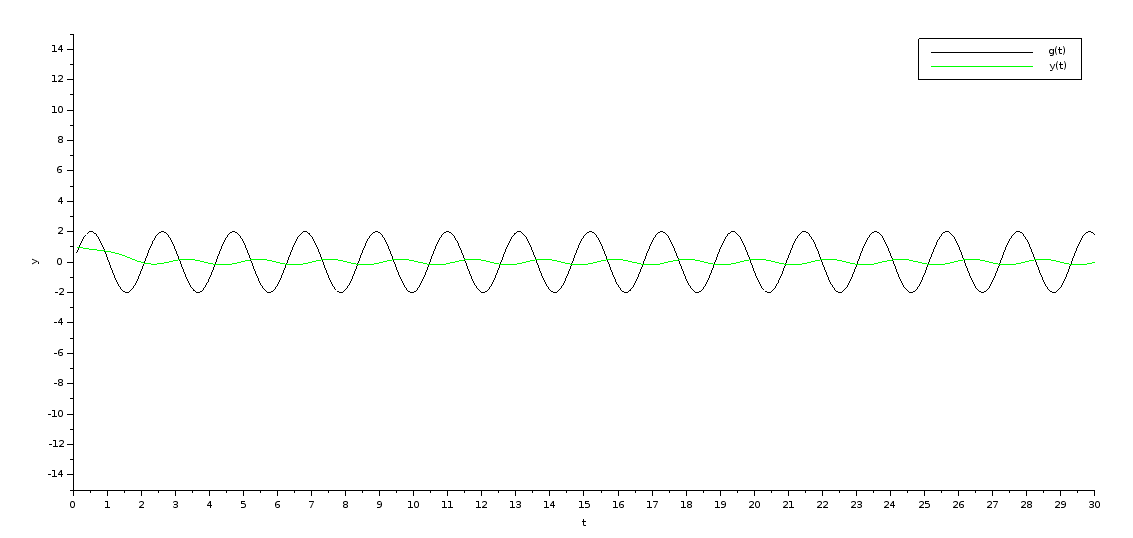
\includegraphics[width=0.9\textwidth]{3g1.png}
\end{center}



\section{Выводы}

В результате проделанной работы мы смоделировали дифференциальные уравнения вида
$y'' + a_1 y' + a_0 y = bg(t)$, где $b$ может быть равен $0$, что соответствует
свободному движению системы, путём построения аналоговых электрических систем,
описываемых такими дифференциальными уравнениями. Это позволяет осуществлять, к
примеру, анализ затухающих колебательных движений.

\end{document}

